%%%%%%%%%%%%%%%%%%%%%%%%%%%%%%%%
% Compile with
% pdflatex --shell-escape -synctex=1 -interaction=nonstopmode energyLinePath.tex
% to convert it to png use:
% convert -density 300 -transparent white energyLinePath.pdf energyLinePath.png
%%%%%%%%%%%%%%%%%%%%%%%%%%%%%%%%

\documentclass{standalone}

\usepackage[utf8]{inputenc}
\usepackage{tkz-fct}
\renewcommand{\familydefault}{\sfdefault}
\usepackage[scaled=1]{helvet}
\usepackage[helvet]{sfmath}
\everymath={\sf}
\usetikzlibrary{calc,arrows,intersections,angles,quotes,patterns}

\definecolor{AFLight}{HTML}{5CE0E6}
\definecolor{AFMiddle}{HTML}{51ADE5}
\definecolor{AFDark}{HTML}{0E4160}

\begin{document}

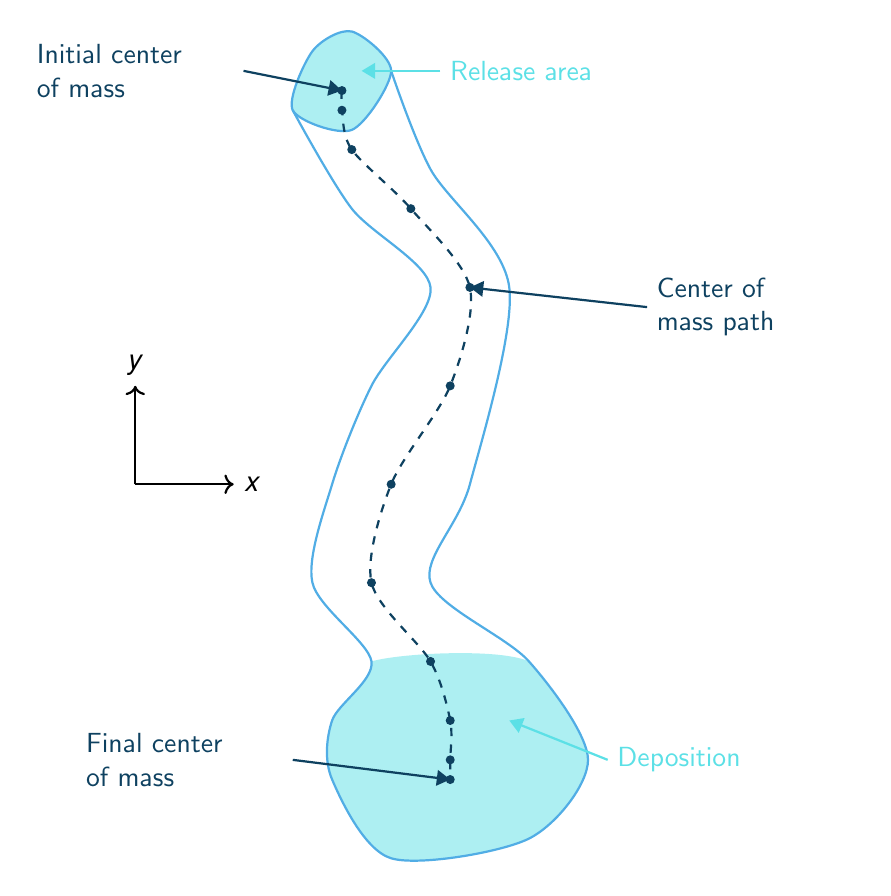
\begin{tikzpicture}[
    scale=0.25,
    point/.style = {draw, circle,  fill = black, inner sep = 1pt},
    dot/.style   = {draw, circle,  fill = black, inner sep = .2pt},
  ]
% defining coordinates
% reference
\coordinate (RR1) at (-2,29);
\coordinate (RR2) at (-1,32);
\coordinate (RR3) at (1,33);
\coordinate (RR4) at (3,31);
\coordinate (RR5) at (1,28);

\coordinate (R1) at (1,24);
\coordinate (R2) at (5,20);
\coordinate (R3) at (2,15);
\coordinate (R4) at (0,10);
\coordinate (R5) at (-1,5);
\coordinate (R6) at (2,1);
\coordinate (R7) at (0,-2);
\coordinate (R8) at (0,-5);
\coordinate (R9) at (3,-9);
\coordinate (R10) at (10,-8);
\coordinate (R11) at (13,-4);
\coordinate (R12) at (10,1);
\coordinate (R13) at (5,5);
\coordinate (R14) at (7,10);
\coordinate (R15) at (9,20);
\coordinate (R16) at (5,26);



% avaPath
\coordinate (O1) at (0.5,30);
\coordinate (O2) at (0.5,29);
\coordinate (O3) at (1,27);
\coordinate (O4) at (4,24);
\coordinate (O5) at (7,20);
\coordinate (O6) at (6,15);
\coordinate (O7) at (3,10);
\coordinate (O8) at (2,5);
\coordinate (O9) at (5,1);
\coordinate (O10) at (6,-2);
\coordinate (O11) at (6,-4);
\coordinate (O12) at (6,-5);
\coordinate (O11) at (6,-4);
\coordinate (O10) at (6,-2);
\coordinate (O9) at (5,1);
\coordinate (O8) at (2,5);
\coordinate (O7) at (3,10);
\coordinate (O6) at (6,15);
\coordinate (O4) at (4,24);


\def\RefAvaRel{
     plot [smooth cycle] coordinates {(RR1) (RR2) (RR3) (RR4) (RR5)}
    }
\def\RefAva{
      plot [smooth] coordinates {(RR1) (R1) (R2) (R3) (R4) (R5) (R6) (R7)  (R8) (R9) (R10) (R11)  (R12) (R13)  (R14)  (R15) (R16) (RR4)}
    }
\def\DepAva{
      plot [smooth cycle] coordinates {(R6) (R7)  (R8) (R9) (R10) (R11)  (R12)}
    }
\def\AvaPath{
     plot [smooth] coordinates {(O1) (O2) (O3) (O4) (O5) (O6) (O7) (O8) (O9) (O10) (O11) (O12)}
    }


\begin{scope}
      \clip \RefAva;
      \clip \DepAva; %(-5,-10) rectangle (15,0);
      \fill[AFLight!50] \RefAva;
\end{scope}

\draw [thick, AFMiddle, fill=AFLight!50] \RefAvaRel;
\draw [thick, AFMiddle] \RefAva ;


\draw [thick, dashed, AFDark] \AvaPath;
 \foreach \point in {(O1), (O2), (O3), (O4), (O5), (O6), (O7), (O8), (O9), (O10), (O11), (O12)}
 {
      \node[point, AFDark] at \point {};

    }



\draw [thick, black, ->] (-10,10) -- (-5,10) node[right] {$x$};
\draw [thick, black, ->] (-10,10) -- (-10,15) node[above] {$y$};


\node[text width=2.5cm, fill=none, right, AFDark] at ($(O5) +(9,-1)$) {Center of \\ mass path};
\draw [>={Triangle},thick, ->, AFDark] ($(O5) +(9,-1)$) -- (O5) ;


\node[text width=2.5cm, fill=none, right, AFLight] at ($(O1) +(5,1)$) {Release area};
\draw [>={Triangle},thick, ->, AFLight] ($(O1) +(5,1)$) -- ($(O1) +(1,1)$) ;
\node[text width=2.5cm, fill=none, left, AFDark] at ($(O1) +(-5,1)$) {Initial center\\ of mass};
\draw [>={Triangle},thick, ->, AFDark] ($(O1) +(-5,1)$) -- (O1) ;

\node[text width=2.5cm, fill=none, right, AFLight] at ($(O12) +(8,1)$) {Deposition};
\draw [>={Triangle},thick, ->, AFLight] ($(O12) +(8,1)$) -- ($(O12) +(3,3)$) ;

\node[text width=2.5cm, fill=none, left, AFDark] at ($(O12) +(-8,1)$) {Final center \\ of mass};
\draw [>={Triangle},thick, ->, AFDark] ($(O12) +(-8,1)$) -- (O12);


\end{tikzpicture}

\end{document}
